\documentclass[]{book}
\usepackage{lmodern}
\usepackage{amssymb,amsmath}
\usepackage{ifxetex,ifluatex}
\usepackage{fixltx2e} % provides \textsubscript
\ifnum 0\ifxetex 1\fi\ifluatex 1\fi=0 % if pdftex
  \usepackage[T1]{fontenc}
  \usepackage[utf8]{inputenc}
\else % if luatex or xelatex
  \ifxetex
    \usepackage{mathspec}
  \else
    \usepackage{fontspec}
  \fi
  \defaultfontfeatures{Ligatures=TeX,Scale=MatchLowercase}
\fi
% use upquote if available, for straight quotes in verbatim environments
\IfFileExists{upquote.sty}{\usepackage{upquote}}{}
% use microtype if available
\IfFileExists{microtype.sty}{%
\usepackage{microtype}
\UseMicrotypeSet[protrusion]{basicmath} % disable protrusion for tt fonts
}{}
\usepackage{hyperref}
\hypersetup{unicode=true,
            pdftitle={EMVS: The EM Approach to Bayesian Variable Selection},
            pdfauthor={Caleb Jin},
            pdfborder={0 0 0},
            breaklinks=true}
\urlstyle{same}  % don't use monospace font for urls
\usepackage{natbib}
\bibliographystyle{apalike}
\usepackage{color}
\usepackage{fancyvrb}
\newcommand{\VerbBar}{|}
\newcommand{\VERB}{\Verb[commandchars=\\\{\}]}
\DefineVerbatimEnvironment{Highlighting}{Verbatim}{commandchars=\\\{\}}
% Add ',fontsize=\small' for more characters per line
\usepackage{framed}
\definecolor{shadecolor}{RGB}{248,248,248}
\newenvironment{Shaded}{\begin{snugshade}}{\end{snugshade}}
\newcommand{\AlertTok}[1]{\textcolor[rgb]{0.94,0.16,0.16}{#1}}
\newcommand{\AnnotationTok}[1]{\textcolor[rgb]{0.56,0.35,0.01}{\textbf{\textit{#1}}}}
\newcommand{\AttributeTok}[1]{\textcolor[rgb]{0.77,0.63,0.00}{#1}}
\newcommand{\BaseNTok}[1]{\textcolor[rgb]{0.00,0.00,0.81}{#1}}
\newcommand{\BuiltInTok}[1]{#1}
\newcommand{\CharTok}[1]{\textcolor[rgb]{0.31,0.60,0.02}{#1}}
\newcommand{\CommentTok}[1]{\textcolor[rgb]{0.56,0.35,0.01}{\textit{#1}}}
\newcommand{\CommentVarTok}[1]{\textcolor[rgb]{0.56,0.35,0.01}{\textbf{\textit{#1}}}}
\newcommand{\ConstantTok}[1]{\textcolor[rgb]{0.00,0.00,0.00}{#1}}
\newcommand{\ControlFlowTok}[1]{\textcolor[rgb]{0.13,0.29,0.53}{\textbf{#1}}}
\newcommand{\DataTypeTok}[1]{\textcolor[rgb]{0.13,0.29,0.53}{#1}}
\newcommand{\DecValTok}[1]{\textcolor[rgb]{0.00,0.00,0.81}{#1}}
\newcommand{\DocumentationTok}[1]{\textcolor[rgb]{0.56,0.35,0.01}{\textbf{\textit{#1}}}}
\newcommand{\ErrorTok}[1]{\textcolor[rgb]{0.64,0.00,0.00}{\textbf{#1}}}
\newcommand{\ExtensionTok}[1]{#1}
\newcommand{\FloatTok}[1]{\textcolor[rgb]{0.00,0.00,0.81}{#1}}
\newcommand{\FunctionTok}[1]{\textcolor[rgb]{0.00,0.00,0.00}{#1}}
\newcommand{\ImportTok}[1]{#1}
\newcommand{\InformationTok}[1]{\textcolor[rgb]{0.56,0.35,0.01}{\textbf{\textit{#1}}}}
\newcommand{\KeywordTok}[1]{\textcolor[rgb]{0.13,0.29,0.53}{\textbf{#1}}}
\newcommand{\NormalTok}[1]{#1}
\newcommand{\OperatorTok}[1]{\textcolor[rgb]{0.81,0.36,0.00}{\textbf{#1}}}
\newcommand{\OtherTok}[1]{\textcolor[rgb]{0.56,0.35,0.01}{#1}}
\newcommand{\PreprocessorTok}[1]{\textcolor[rgb]{0.56,0.35,0.01}{\textit{#1}}}
\newcommand{\RegionMarkerTok}[1]{#1}
\newcommand{\SpecialCharTok}[1]{\textcolor[rgb]{0.00,0.00,0.00}{#1}}
\newcommand{\SpecialStringTok}[1]{\textcolor[rgb]{0.31,0.60,0.02}{#1}}
\newcommand{\StringTok}[1]{\textcolor[rgb]{0.31,0.60,0.02}{#1}}
\newcommand{\VariableTok}[1]{\textcolor[rgb]{0.00,0.00,0.00}{#1}}
\newcommand{\VerbatimStringTok}[1]{\textcolor[rgb]{0.31,0.60,0.02}{#1}}
\newcommand{\WarningTok}[1]{\textcolor[rgb]{0.56,0.35,0.01}{\textbf{\textit{#1}}}}
\usepackage{longtable,booktabs}
\usepackage{graphicx,grffile}
\makeatletter
\def\maxwidth{\ifdim\Gin@nat@width>\linewidth\linewidth\else\Gin@nat@width\fi}
\def\maxheight{\ifdim\Gin@nat@height>\textheight\textheight\else\Gin@nat@height\fi}
\makeatother
% Scale images if necessary, so that they will not overflow the page
% margins by default, and it is still possible to overwrite the defaults
% using explicit options in \includegraphics[width, height, ...]{}
\setkeys{Gin}{width=\maxwidth,height=\maxheight,keepaspectratio}
\IfFileExists{parskip.sty}{%
\usepackage{parskip}
}{% else
\setlength{\parindent}{0pt}
\setlength{\parskip}{6pt plus 2pt minus 1pt}
}
\setlength{\emergencystretch}{3em}  % prevent overfull lines
\providecommand{\tightlist}{%
  \setlength{\itemsep}{0pt}\setlength{\parskip}{0pt}}
\setcounter{secnumdepth}{5}
% Redefines (sub)paragraphs to behave more like sections
\ifx\paragraph\undefined\else
\let\oldparagraph\paragraph
\renewcommand{\paragraph}[1]{\oldparagraph{#1}\mbox{}}
\fi
\ifx\subparagraph\undefined\else
\let\oldsubparagraph\subparagraph
\renewcommand{\subparagraph}[1]{\oldsubparagraph{#1}\mbox{}}
\fi

%%% Use protect on footnotes to avoid problems with footnotes in titles
\let\rmarkdownfootnote\footnote%
\def\footnote{\protect\rmarkdownfootnote}

%%% Change title format to be more compact
\usepackage{titling}

% Create subtitle command for use in maketitle
\providecommand{\subtitle}[1]{
  \posttitle{
    \begin{center}\large#1\end{center}
    }
}

\setlength{\droptitle}{-2em}

  \title{EMVS: The EM Approach to Bayesian Variable Selection}
    \pretitle{\vspace{\droptitle}\centering\huge}
  \posttitle{\par}
    \author{Caleb Jin}
    \preauthor{\centering\large\emph}
  \postauthor{\par}
      \predate{\centering\large\emph}
  \postdate{\par}
    \date{12-15-2017}

\usepackage{booktabs}

\begin{document}
\maketitle

{
\setcounter{tocdepth}{1}
\tableofcontents
}
\hypertarget{foreword}{%
\chapter{Foreword}\label{foreword}}

I am \href{https://www.sjin.name/}{Caleb Jin}. After I read this paper, \textbf{\href{https://www.tandfonline.com/doi/full/10.1080/01621459.2013.869223}{EMVS: The EM Approach to Bayesian Variable Selection}}\citep{EMVS}, I write down the nodes of the key idea and R code to realize it.

\newcommand\T{{\top}}
\newcommand\ubeta{{\boldsymbol \beta}}
\newcommand\uSigma{{\boldsymbol \Sigma}}
\newcommand\uepsilon{{\boldsymbol \epsilon}}
\newcommand\umu{{\boldsymbol \mu}}
\newcommand\utheta{{\boldsymbol \theta}}
\newcommand\bg{{\boldsymbol \gamma}}
\newcommand\uphi{{\boldsymbol \phi}}
\newcommand\0{{\bf 0}}
\newcommand\uX{{\bf X}}
\newcommand\uD{{\bf D}}
\newcommand\ux{{\bf x}}
\newcommand\uY{{\bf Y}}
\newcommand\uy{{\bf y}}
\newcommand\uz{{\bf z}}
\newcommand\uI{{\bf I}}
\newcommand\uA{{\bf A}}
\newcommand\uB{{\bf B}}
\newcommand\uH{{\bf H}}
\newcommand\uM{{\bf M}}
\newcommand\uV{{\bf V}}
\newcommand\diag{{\rm diag}}

\hypertarget{the-em-approach-to-bayesian-variable-selection}{%
\chapter{The EM Approach to Bayesian Variable Selection}\label{the-em-approach-to-bayesian-variable-selection}}

\hypertarget{introduction}{%
\section{Introduction}\label{introduction}}

The \textbf{EMVS} method is anchored by \textbf{EM} algorithm and original stochastic search variable selection (\textbf{SSVS}). It is a deterministic alternative to \textbf{MCMC} stochastic search and ideally suited for high-dimensional \(p>n\) settings. Furthermore, \textbf{EMVS} is able to effectively identify the sparse high-probability model and find candidate models within a fraction of the time needed by \textbf{SSVS}. This algorithm makes it possible to carry out dynamic posterior exploration for the identification of posterior modes.

The outline of this course project is as follows. In section 2, we build original \textbf{SSVS} method, including its prior and posterior distribution for each parameter. In section 3, I derive the author's new idea \textbf{EMVS} method in very details that the author omits. In section 4, I perform several simulation case studies from this paper and me, then compare the results of \textbf{SSVS} and \textbf{EMVS}.

\hypertarget{stochastic-search-variable-selection-ssvs}{%
\section{Stochastic Search Variable Selection (SSVS)}\label{stochastic-search-variable-selection-ssvs}}

\hypertarget{model-settings}{%
\subsection{Model Settings}\label{model-settings}}

Consider a multiple linear regression model as follows:
\begin{eqnarray}
    {\bf y}={\bf X}{\boldsymbol \beta}+ {\boldsymbol \epsilon},
    \label{eq:1}
    \end{eqnarray}
where \({\bf y}=(y_1,\ldots,y_n)^{{\top}}\) is the \(n\)-dimensional response vector, \({\bf X}=[{\bf x}_1,\ldots,{\bf x}_n]^{{\top}}\) is the \(n\times p\) design
matrix, \({\boldsymbol \beta}=(\beta_1, \beta_2, \ldots, \beta_p)'\), \(\sigma^2\) is a scalar, and \({\boldsymbol \epsilon}\sim \mathcal{N}_n({\bf 0},\sigma^2{\bf I}_n)\).
Both \(\sigma^2\) and \({\boldsymbol \beta}\) are considerd bo te unknown. We assume that \(p>n\).
From \eqref{eq:1}, the likelihood function is given as
\begin{eqnarray}
    {\bf y}|{\boldsymbol \beta}, \sigma^2 \sim \mathcal{N}({\bf X}{\boldsymbol \beta}, \sigma^2I_n).
    \end{eqnarray}

\subsection{Prior Specification}

The cornerstone of \(\textbf{SSVS}\) is the ``spike and slab'' Gaussian mixture prior on \({\boldsymbol \beta}\),
\begin{eqnarray}
    \beta_j|\sigma^2,\gamma_j \stackrel{ind}{\sim} (1-\gamma_j) \mathcal{N}(0, \sigma^2\nu_0) + \gamma_j\mathcal{N}(0,\sigma^2\nu_1),
    \end{eqnarray}
where
\begin{eqnarray*}
        \gamma_j=\left\{
        \begin{array}{lcr}
            1 & \beta_j \neq 0\\
            0 & \beta_j=0,
\end{array}\right.
\label{eq:spike-slab}
\end{eqnarray*}
\(j=1,2,\ldots, p\). \(0\leq \nu_0<\nu_1\).\textbackslash{}
Hence, \({\boldsymbol \beta}|\sigma^2,{\boldsymbol \gamma}\sim \mathcal{N}_p({\bf 0},{\bf D}_{\sigma^2,{\boldsymbol \gamma}})\), where \({\bf D}_{\sigma^2,{\boldsymbol \gamma}} = \sigma^2  {\rm diag}(\nu_{z_1},\nu_{z_1},\ldots,\nu_{z_p})\).\textbackslash{}
For the prior on the \(\sigma^2\), I follow the GM97 and use inverse gamma prior but different notation,
\begin{eqnarray}
    \sigma^2 \sim \mathcal{IG}(\frac{a}{2}, \frac{b}{2}),
    \end{eqnarray}
where we will use \(a=1\) and \(b=1\), and \(\sigma^2\) is also independent of \({\boldsymbol \gamma}\). \textbackslash{}
I follow the GM97 and use Bernoulli prior form but different notation,
\begin{eqnarray}
    \gamma_j|\theta \stackrel{iid}{\sim} Ber(\theta), \theta \in [0,1].
    \end{eqnarray}
Hence,
\begin{eqnarray}\label{gamma}
    {\boldsymbol \gamma}\propto \theta^{\sum_{j=1}^{p}\gamma_j}(1-\theta)^{p-\sum_{j=1}^{p}\gamma_j} 
    \label{eq:gamma}
    \end{eqnarray}
We assume
\begin{eqnarray}
    \theta \sim \mathcal{B}(c_1,c_2),
    \end{eqnarray}
where we will use \(c_1=c_2=1\), which leads to the uniform distribution.\textbackslash{}

It is easy to show that the full conditionals are as follows:

\begin{itemize}
\item
  \begin{enumerate}
  \def\labelenumi{\arabic{enumi})}
  \tightlist
  \item
    \[\beta_j|{\boldsymbol \beta}_{-j}, \sigma^2, {\boldsymbol \gamma}, \nu_0, {\bf y}\sim \mathcal{N}(\tilde{\beta}_j, \frac{\sigma^2}{\mu_j}).\]
    where \(\mu_j= x_j^{{\top}}x_j + \frac{1}{\nu_{\gamma_j}}\) and \(\tilde{\beta}_j = \mu_j^{-1}x_j^{{\top}}({\bf y}- {\bf X}_{-j}{\boldsymbol \beta}_{-j})\).
  \end{enumerate}
\item
  \begin{enumerate}
  \def\labelenumi{\arabic{enumi})}
  \setcounter{enumi}{1}
  \tightlist
  \item
    \begin{eqnarray}
        \gamma_j |{\boldsymbol \gamma}_{-j}, {\boldsymbol \beta}, \sigma^2, {\bf y}\sim Ber\left(\frac{ \nu_1^{-\frac{1}{2}}
            \exp\left(-\frac{1}{2\sigma^2\nu_1}\beta_j^2\right)\theta}
        {  \nu_0^{-\frac{1}{2}}\exp\left(-\frac{1}{2\sigma^2\nu_0}\beta_j^2\right)\left(1-\theta\right)+
            \nu_1^{-\frac{1}{2}}\exp\left(-\frac{1}{2\sigma^2\nu_1}\beta_j^2\right)\theta}\right).
    \end{eqnarray}
  \end{enumerate}
\item
  \begin{enumerate}
  \def\labelenumi{\arabic{enumi})}
  \setcounter{enumi}{2}
  \tightlist
  \item
    \[\sigma^2|{\boldsymbol \beta}, {\boldsymbol \gamma}, {\bf y}\sim \mathcal{IG}(a^*,b^*).\]
    where \(a^*=\frac{1}{2}(n+p+a)\) and \(b^* = \frac{1}{2}\left(\|{\bf y}-{\bf X}{\boldsymbol \beta}\|^2 + \sum_{j=1}^{p}\frac{\beta_j^2}{\nu_{\gamma_j}} + b\right).\)
  \end{enumerate}
\item
  \begin{enumerate}
  \def\labelenumi{\arabic{enumi})}
  \setcounter{enumi}{3}
  \tightlist
  \item
    For \(\theta|{\boldsymbol \gamma}\), we have
  \end{enumerate}
\end{itemize}

\begin{align}
        \pi(\theta|{\boldsymbol \gamma})&\propto \pi({\boldsymbol \gamma}|\theta) \pi(\theta) \nonumber \\
        &\propto\left[ \prod_{j=1}^p \theta^{\gamma_j}(1-\theta)^{1-\gamma_j}\right] \theta^{c_1-1}(1-\theta)^{c_2-1} \nonumber\\
        &\propto \theta^{\sum_{j=1}^p \gamma_j+c_1-1}(1-\theta)^{p-\sum_{j=1}^p \gamma_j+c_2-1},
\end{align}
where we will use \(c_1=c_2=1\), which leads to the uniform distribution.
We therefore have
\begin{eqnarray}
        \theta|{\boldsymbol \gamma}\sim \mathcal{B}\left(\sum_{j=1}^p \gamma_j+c_1,p-\sum_{j=1}^p \gamma_j+c_2\right).
\end{eqnarray}

\hypertarget{emvs}{%
\section{EMVS}\label{emvs}}

Genared toward finding posterior modes of the parameter posterior \(\pi({\boldsymbol \beta},\sigma^2,\theta|{\bf y})\) rather than simulating from the entire model posterior \(\pi({\boldsymbol \gamma}|{\bf y})\), the EM algorithm derived here offers potentially enormous computational savings over stochastic search alternatives, especially in problems with a large number p of potential predictors.

\(\textbf{EMVS}\) consists of two steps: E-Step, conditional expectation given the observed data and current parameter estimates, and M-Step, entails the maximization of the expected complete data log posterior with respect to \(({\boldsymbol \beta},\sigma^2,\theta)\).

Define \({\boldsymbol \phi}= ({\boldsymbol \beta},\sigma^2,\theta)\). EM algorithm maximizes \(\pi({\boldsymbol \phi}|{\bf y})\) by iteratively maximizing the objective function
\begin{eqnarray*}
        Q({\boldsymbol \phi}|{\boldsymbol \phi}^{(t-1)},{\bf y}) = E_{{\boldsymbol \gamma}|\cdot}[\log \pi({\boldsymbol \phi},{\boldsymbol \gamma}|{\bf y})],
\end{eqnarray*}
where \(E_{{\boldsymbol \gamma}|\cdot}\) denotes \(E_{{\boldsymbol \gamma}|{\boldsymbol \phi}^{(t-1)},{\bf y}}\).

According to the class note, it can be written as
\begin{eqnarray}
    Q^{\star}({\boldsymbol \phi}|{\boldsymbol \phi}^{(t-1)},{\bf y}) = E_{{\boldsymbol \gamma}|\cdot}[\log \pi({\boldsymbol \phi}|{\boldsymbol \gamma},{\bf y})]
    \label{eq:Estep}
\end{eqnarray}
At the \((t-1)\)th iteration, given \({\boldsymbol \phi}^{(t-1)}\), an E-step is first applied, which computes the expectation of the right side of \eqref{eq:Estep} to obtain \(Q\). This is followed by M-step, which maximizes \(Q\) over \(({\boldsymbol \beta},\sigma^2,\theta)\) to obtain \(({\boldsymbol \beta}^{(t)},\sigma^{2{(t)}},\theta^{(t)})\).

\begin{eqnarray*}
        &&Q^{\star}({\boldsymbol \beta},\sigma^2,\theta|{\boldsymbol \beta}^{(t)},\sigma^{2{(t)}},\theta^{(t)},{\bf y}) \\
        &=& Q^{\star}({\boldsymbol \beta},\sigma^2,\theta|{\boldsymbol \phi}^{(t-1)},{\bf y}) \\
        &=& C + Q_1({\boldsymbol \beta},\sigma^2|{\boldsymbol \phi}^{(t-1)},{\bf y}) + Q_2(\theta|{\boldsymbol \phi}^{(t-1)},{\bf y})\\
        &=& C + E_{{\boldsymbol \gamma}|\cdot}[\log \pi({\boldsymbol \beta},\sigma^2|{\boldsymbol \phi}^{(t-1)},{\bf y})]+
        E_{{\boldsymbol \gamma}|\cdot}[\log \pi(\theta|{\boldsymbol \phi}^{(t-1)},{\bf y})]
\end{eqnarray*}

\begin{itemize}
\item
  \begin{enumerate}
  \def\labelenumi{(\arabic{enumi})}
  \tightlist
  \item
    \(Q_1({\boldsymbol \beta},\sigma^2|{\boldsymbol \phi}^{(t-1)},{\bf y})\)
    \begin{eqnarray*}
          &&\pi({\boldsymbol \beta},\sigma^2|{\boldsymbol \phi}^{(t-1)},{\bf y})\\
          &\propto& \pi(y|{\boldsymbol \beta},\sigma^2)\pi({\boldsymbol \beta}|\sigma^2,{\boldsymbol \gamma})\pi(\sigma^2)\\
          &\propto& (\sigma^2)^{-\frac{n}{2}}\exp\left(-\frac{1}{2\sigma^2}||y-x{\boldsymbol \beta}||^2\right)
          (\sigma^2)^{-\frac{p}{2}}\prod_{j=1}^{p}\nu_{\gamma_j}\exp\left(-\frac{1}{2\sigma^2\nu_{\gamma_j}}\beta_j^2\right)\\
          &&\times (\sigma^2)^{-\frac{a}{2}-1}\exp\left(-\frac{b}{2\sigma^2}\right)\\
          &\propto& (\sigma^2)^{-\frac{n+p+a+2}{2}}\exp\left[-\frac{1}{2\sigma^2}\left(||y-x{\boldsymbol \beta}||^2+
          \sum_{j=1}^{p}\beta_j^2\frac{1}{\nu_{\gamma_j}}+b\right)\right]
    \end{eqnarray*}
  \end{enumerate}
\end{itemize}

\begin{eqnarray*}
            &&Q_1({\boldsymbol \beta},\sigma^2|{\boldsymbol \phi}^{(t-1)},{\bf y})\\
            &=& E_{{\boldsymbol \gamma}|\cdot}[\log(\pi({\boldsymbol \beta},\sigma^2|{\boldsymbol \phi}^{(t-1)},{\bf y}))]\\
            &=& -\frac{1}{2}(n+p+a+2)\log(\sigma^2)-\frac{1}{2\sigma^2}(||y-x{\boldsymbol \beta}||^2+b)-\frac{1}{2\sigma^2}
            \sum_{j=1}^{p}\beta_j^2E_{{\boldsymbol \gamma}|\cdot}[\frac{1}{\nu_{\gamma_j}}]
\end{eqnarray*}

\begin{itemize}
\item
  \begin{enumerate}
  \def\labelenumi{(\arabic{enumi})}
  \setcounter{enumi}{1}
  \tightlist
  \item
    \(Q_2(\theta|{\boldsymbol \phi}^{(t-1)},{\bf y})\)
    \begin{eqnarray*}
          &&\pi(\theta|{\boldsymbol \gamma},{\bf y})\\
          &\propto& \pi({\boldsymbol \gamma}|\theta)p(\theta)\\
          &\propto& \theta^{\sum_{j=1}^{p}\gamma_j+c_1-1}(1-\theta)^{p-\sum_{j=1}^{p}\gamma_j+c_2-1}
    \end{eqnarray*}
  \end{enumerate}
\end{itemize}

\begin{eqnarray*}
            &&\log(\pi(\theta|{\boldsymbol \gamma},{\bf y}))\\
            &=& C+ (\sum_{j=1}^{p}\gamma_j+c_1-1)\log \theta + (p-\sum_{j=1}^{p}\gamma_j+c_2-1)\log
            (1-\theta)\\        
            &=& C+\log \frac{\theta}{1-\theta} \sum_{j=1}^{p}\gamma_j
            + (c_1-1)\log\theta + (p+c_2-1)\log(1-\theta)   
\end{eqnarray*}

\begin{eqnarray*}
            &&Q_2(\theta|{\boldsymbol \phi}^{(t-1)},{\bf y})\\
            &=& \log \frac{\theta}{1-\theta} \sum_{j=1}^{p}E_{{\boldsymbol \gamma}|\cdot}[\gamma_j]+
            (c_1-1)\log\theta + (p+c_2-1)\log(1-\theta) \\
\end{eqnarray*}

\hypertarget{the-e-step}{%
\subsection{The E-Step}\label{the-e-step}}

The E-step proceeds by computing the conditional expectations \(E_{{\boldsymbol \gamma}|\cdot}[\frac{1}{\nu_{\gamma_j}}]\) and \(E_{{\boldsymbol \gamma}|\cdot}[\gamma_j]\) for \(Q_1\) and \(Q_2\), respectively.

\begin{itemize}
\item
  \begin{enumerate}
  \def\labelenumi{(\arabic{enumi})}
  \tightlist
  \item
    For \(E_{{\boldsymbol \gamma}|\cdot}[\gamma_j]\),
  \end{enumerate}
\end{itemize}

\begin{eqnarray*}
            &&\pi(\gamma_j|\theta,\beta_j,\sigma^2,{\bf y})\\
            &\propto&\pi(\beta_j|\gamma_j,\sigma^2)p(\gamma_j|\theta)\\
            &\propto&\nu_{\gamma_j}^{-\frac{1}{2}}\exp\left(-\frac{1}{2\sigma^2\nu_{\gamma_j}}\beta_j^2\right)
            \theta^{\gamma_j}(1-\theta)^{1-\gamma_j}
\end{eqnarray*}

Hence, \(\pi(\gamma_j=1|\theta,\beta_j,\sigma^2,{\bf y})=C \nu_{1}^{-\frac{1}{2}}\exp\left(-\frac{1}{2\sigma^2\nu_{1}}\beta_j^2\right)\theta\equiv a_i\),

\(\pi(\gamma_j=0|\theta,\beta_j,\sigma^2,{\bf y})=C \nu_{0}^{-\frac{1}{2}}\exp\left(-\frac{1}{2\sigma^2\nu_{0}}\beta_j^2\right)(1-\theta)\equiv b_i\).

Hence,

\begin{eqnarray*}
            &&E_{{\boldsymbol \gamma}|\cdot}[\gamma_j]=\pi(\gamma_j=1|\theta,\beta_j,\sigma^2,{\bf y})\\
            &=&\frac{\pi(\gamma_j=1,\Omega)}{\sum_{\gamma_j}\pi(\gamma_j,\Omega)}\\
            &=&\frac{C \nu_{1}^{-\frac{1}{2}}\exp\left(-\frac{1}{2\sigma^2\nu_{1}}\beta_j^2\right)\theta}
            {C \nu_{1}^{-\frac{1}{2}}\exp\left(-\frac{1}{2\sigma^2\nu_{1}}\beta_j^2\right)\theta
                +C \nu_{0}^{-\frac{1}{2}}\exp\left(-\frac{1}{2\sigma^2\nu_{0}}\beta_j^2\right)(1-\theta)}\\
            &=&\frac{ \nu_{1}^{-\frac{1}{2}}\exp\left(-\frac{1}{2\sigma^2\nu_{1}}\beta_j^2\right)\theta}
            {\nu_{1}^{-\frac{1}{2}}\exp\left(-\frac{1}{2\sigma^2\nu_{1}}\beta_j^2\right)\theta
                + \nu_{0}^{-\frac{1}{2}}\exp\left(-\frac{1}{2\sigma^2\nu_{0}}\beta_j^2\right)(1-\theta)}\\
            &=&p_i^*
\end{eqnarray*}

Hence,

\begin{eqnarray}
        &&Q_2(\theta|{\boldsymbol \phi}^{(t-1)},{\bf y})\nonumber\\
        &=& \log \frac{\theta}{1-\theta} \sum_{j=1}^{p}p_i^*+
        (c_1-1)\log\theta + (p+c_2-1)\log(1-\theta)
        \label{eq:q2}
\end{eqnarray}

\begin{itemize}
\item
  \begin{enumerate}
  \def\labelenumi{(\arabic{enumi})}
  \setcounter{enumi}{1}
  \tightlist
  \item
    For \(E_{{\boldsymbol \gamma}|\cdot}[\frac{1}{\nu_{\gamma_j}}]\),
    \begin{eqnarray*}   
          &&E_{{\boldsymbol \gamma}|\cdot}[\frac{1}{\nu_{\gamma_j}}]\\
          &=&p(\gamma_j=1|\cdot)\frac{1}{\nu_{\gamma_j=1}} +
          p(\gamma_j=0|\cdot)\frac{1}{\nu_{\gamma_j=0}}\\
          &=& \frac{p_i^*}{\nu_{1}}+\frac{1-p_i^*}{\nu_{0}} \equiv d^*_i 
    \end{eqnarray*}
    Hence,
    \begin{eqnarray}
      &&Q_1({\boldsymbol \beta},\sigma^2|{\boldsymbol \phi}^{(t-1)},{\bf y})\nonumber\\
      &=& -\frac{1}{2}(n+p+a+2)\log(\sigma^2)-\frac{1}{2\sigma^2}(||{\bf y}-x{\boldsymbol \beta}||^2+b)-\frac{1}{2\sigma^2}
      \sum_{j=1}^{p}\beta_j^2d^*_i \nonumber\\
      &=& -\frac{1}{2}(n+p+a+2)\log(\sigma^2)-\frac{1}{2\sigma^2}(||{\bf y}-x{\boldsymbol \beta}||^2+b)-\nonumber\\
      &&\frac{1}{2\sigma^2} ||{\bf D}^{*1/2}{\boldsymbol \beta}||^2, 
      \label{eq:q1}
    \end{eqnarray}
    where \({\bf D}^*={\rm diag}\{d_i^*\}_{i=1}^{p^*}\)
  \end{enumerate}
\end{itemize}

\hypertarget{the-m-step}{%
\subsection{The M-Step}\label{the-m-step}}

\begin{itemize}
\item
  \begin{enumerate}
  \def\labelenumi{(\arabic{enumi})}
  \item
    Maximize \(Q_1\)

    \({\boldsymbol \beta}\) values that maximizes \(Q1\) in Eq.\eqref{eq:q1} is equivalent to
    \[
      {\boldsymbol \beta}^{(t)}=\arg\min_{{\boldsymbol \beta}\to\mathcal{R}^p}||{\bf y}-x{\boldsymbol \beta}||^2+||{\bf D}^{*1/2}{\boldsymbol \beta}||^2.
      \]
    This is quickly obtained by the well-known solution to the ridge regression problem:
    \[
      {\boldsymbol \beta}^{(t)} = ({\bf X}^{{\top}}{\bf X}+{\bf D}^*)^{-1}{\bf X}^{{\top}}{\bf y}
      \]

    Given \({\boldsymbol \beta}^{(t)}\), solve the solution of \(\frac{\partial Q_1}{\partial \sigma^2}\), we can easily obtain
    \[
      \sigma^{2(t)} = \frac{||{\bf y}-{\bf X}{\boldsymbol \beta}^{(t)}||^2+ ||{\bf D}^{*1/2}{\boldsymbol \beta}^{(t)}||^2 + b}{n+p+a+2}.
      \]
  \end{enumerate}
\item
  \begin{enumerate}
  \def\labelenumi{(\arabic{enumi})}
  \setcounter{enumi}{1}
  \tightlist
  \item
    Maximize \(Q_2\)
  \end{enumerate}
\end{itemize}

\begin{eqnarray*}
            &&\frac{\partial Q_2}{\partial \theta}\\
            &=& \frac{1-\theta}{\theta}\frac{1-\theta+\theta}{(1-\theta)^2}\sum_{j=1}^{p}p_j^*+\frac{a-1}{\theta}-\frac{p+b-1}{1-\theta}\\
            &=&\frac{\sum_{j=1}^{p}p_j^*}{\theta(1-\theta)}+\frac{a-1}{\theta}-\frac{p+b-1}{1-\theta}\\
            &=&\frac{\sum_{j=1}^{p}p_j^*-(a+b+p-2)\theta+a-1}{\theta(1-\theta)}\\
            &\equiv& 0
\end{eqnarray*}
Hence, we have \(\theta^{(t)}=\frac{\sum_{j=1}^{p}p_j^*+a-1}{a+b+p-2}\).

\hypertarget{simulation-case-study}{%
\section{Simulation Case Study}\label{simulation-case-study}}

According to this paper, the author simulate a dataset consisting of \(n=100\) observations and \(p=1000\) predictors. Predictor values for each observation were sampled from \(\mathcal{N}_p({\bf 0},{\boldsymbol \Sigma})\) where \({\boldsymbol \Sigma}= (\rho_{ij})_{i,j=1}^p\) with \(\rho_{ij}=0.6^{|i-j|}\). Response values were then generated according to the linear model \({\bf y}={\bf X}{\boldsymbol \beta}+{\boldsymbol \epsilon}\), where \({\boldsymbol \beta}=(3,2,1,0,0,\ldots,0)^{{\top}}\) and \({\boldsymbol \epsilon}\sim \mathcal{N}_n({\bf 0},\sigma^2{\bf I}_n)\) with \(\sigma^2 = 3\).

The R code is shown bellow

\begin{Shaded}
\begin{Highlighting}[]
\KeywordTok{library}\NormalTok{(mvtnorm)}
\KeywordTok{library}\NormalTok{(ggplot2)}
\KeywordTok{library}\NormalTok{(reshape2)}
\NormalTok{n <-}\StringTok{ }\DecValTok{100}
\NormalTok{p <-}\StringTok{ }\DecValTok{1000}
\NormalTok{beta <-}\StringTok{  }\KeywordTok{c}\NormalTok{(}\DecValTok{3}\NormalTok{,}\DecValTok{2}\NormalTok{,}\DecValTok{1}\NormalTok{,}\KeywordTok{rep}\NormalTok{(}\DecValTok{0}\NormalTok{,p}\DecValTok{-3}\NormalTok{))}
\NormalTok{Sigma <-}\StringTok{ }\KeywordTok{matrix}\NormalTok{(}\OtherTok{NA}\NormalTok{,p,p)}
\ControlFlowTok{for}\NormalTok{ (i }\ControlFlowTok{in} \DecValTok{1}\OperatorTok{:}\NormalTok{p) \{}
  \ControlFlowTok{for}\NormalTok{ (j }\ControlFlowTok{in} \DecValTok{1}\OperatorTok{:}\NormalTok{p) \{}
\NormalTok{    Sigma[i,j] =}\StringTok{ }\FloatTok{0.6}\OperatorTok{^}\NormalTok{(}\KeywordTok{abs}\NormalTok{(i}\OperatorTok{-}\NormalTok{j))}
\NormalTok{  \}}
\NormalTok{\}}
\KeywordTok{set.seed}\NormalTok{(}\DecValTok{2144}\NormalTok{)}
\NormalTok{x <-}\StringTok{ }\KeywordTok{matrix}\NormalTok{(}\KeywordTok{rmvnorm}\NormalTok{(n,}\DataTypeTok{mean =} \KeywordTok{rep}\NormalTok{(}\DecValTok{0}\NormalTok{,p), }\DataTypeTok{sigma =}\NormalTok{ Sigma),}\DataTypeTok{nrow =}\NormalTok{ n)}
\NormalTok{y <-}\StringTok{ }\NormalTok{x}\OperatorTok\NormalTok{beta }\OperatorTok{+}\StringTok{ }\KeywordTok{rnorm}\NormalTok{(n,}\DecValTok{0}\NormalTok{,}\KeywordTok{sqrt}\NormalTok{(}\DecValTok{3}\NormalTok{))}
\CommentTok{## prior and initial values}
\NormalTok{MC =}\StringTok{ }\DecValTok{20}
\NormalTok{nu0 =}\StringTok{ }\FloatTok{0.5}
\NormalTok{nu1 <-}\StringTok{ }\DecValTok{1000}
\NormalTok{hat.theta =}\StringTok{ }\KeywordTok{rep}\NormalTok{(}\DecValTok{1}\NormalTok{,MC)}
\NormalTok{hat.theta[}\DecValTok{1}\NormalTok{] =}\StringTok{ }\FloatTok{0.5}
\NormalTok{hat.gamma <-}\StringTok{ }\KeywordTok{rep}\NormalTok{(}\DecValTok{1}\NormalTok{, p)}
\NormalTok{hat.beta =}\StringTok{ }\KeywordTok{matrix}\NormalTok{(}\OtherTok{NA}\NormalTok{,}\DataTypeTok{nrow =}\NormalTok{ MC, }\DataTypeTok{ncol =}\NormalTok{ p)}
\NormalTok{hat.beta[}\DecValTok{1}\NormalTok{,] =}\StringTok{ }\KeywordTok{rep}\NormalTok{(}\DecValTok{1}\NormalTok{,p)}
\NormalTok{hat.sig2 <-}\StringTok{ }\KeywordTok{rep}\NormalTok{(}\OtherTok{NA}\NormalTok{,MC)}
\NormalTok{hat.sig2[}\DecValTok{1}\NormalTok{] <-}\StringTok{ }\DecValTok{1}\CommentTok{#mean((y - x %*% hat.beta[1,])^2)}

\ControlFlowTok{for}\NormalTok{ (i }\ControlFlowTok{in} \DecValTok{2}\OperatorTok{:}\NormalTok{MC) \{}
\NormalTok{  a <-}\StringTok{ }\KeywordTok{dnorm}\NormalTok{(hat.beta[i}\DecValTok{-1}\NormalTok{,],}\DecValTok{0}\NormalTok{,}\DataTypeTok{sd =} \KeywordTok{sqrt}\NormalTok{(hat.sig2[i}\DecValTok{-1}\NormalTok{]}\OperatorTok{*}\NormalTok{nu1))}\OperatorTok{*}\NormalTok{(hat.theta[i}\DecValTok{-1}\NormalTok{])}
\NormalTok{  b <-}\StringTok{ }\KeywordTok{dnorm}\NormalTok{(hat.beta[i}\DecValTok{-1}\NormalTok{,],}\DecValTok{0}\NormalTok{,}\DataTypeTok{sd =} \KeywordTok{sqrt}\NormalTok{(hat.sig2[i}\DecValTok{-1}\NormalTok{]}\OperatorTok{*}\NormalTok{nu0))}\OperatorTok{*}\NormalTok{(}\DecValTok{1}\OperatorTok{-}\NormalTok{hat.theta[i}\DecValTok{-1}\NormalTok{])}
\NormalTok{  p.star =}\StringTok{ }\NormalTok{a}\OperatorTok{/}\NormalTok{(a}\OperatorTok{+}\NormalTok{b)  }
\NormalTok{  D.star <-}\StringTok{ }\KeywordTok{diag}\NormalTok{((}\DecValTok{1}\OperatorTok{-}\NormalTok{p.star)}\OperatorTok{/}\NormalTok{nu0}\OperatorTok{+}\NormalTok{p.star}\OperatorTok{/}\NormalTok{nu1)}
\NormalTok{  D.star}\FloatTok{.5}\NormalTok{ <-}\StringTok{ }\KeywordTok{diag}\NormalTok{(}\KeywordTok{sqrt}\NormalTok{((}\DecValTok{1}\OperatorTok{-}\NormalTok{p.star)}\OperatorTok{/}\NormalTok{nu0}\OperatorTok{+}\NormalTok{p.star}\OperatorTok{/}\NormalTok{nu1))}
\NormalTok{  hat.beta[i,] <-}\StringTok{ }\KeywordTok{solve}\NormalTok{(}\KeywordTok{t}\NormalTok{(x)}\OperatorTok\NormalTok{x}\OperatorTok{+}\NormalTok{D.star)}\OperatorTok\KeywordTok{t}\NormalTok{(x)}\OperatorTok\NormalTok{y}
\NormalTok{  hat.sig2[i] <-}\StringTok{ }\NormalTok{(}\KeywordTok{t}\NormalTok{(y}\OperatorTok{-}\NormalTok{x}\OperatorTok\NormalTok{hat.beta[i,])}\OperatorTok\NormalTok{(y}\OperatorTok{-}\NormalTok{x}\OperatorTok\NormalTok{hat.beta[i,]) }\OperatorTok{+}\StringTok{ }
\StringTok{                    }\KeywordTok{t}\NormalTok{(D.star}\FloatTok{.5}\OperatorTok\NormalTok{hat.beta[i,])}\OperatorTok\NormalTok{(D.star}\FloatTok{.5}\OperatorTok\NormalTok{hat.beta[i,]) }\OperatorTok{+}\StringTok{ }\DecValTok{1}\NormalTok{)}\OperatorTok{/}\NormalTok{(n}\OperatorTok{+}\NormalTok{p}\OperatorTok{+}\DecValTok{1}\OperatorTok{+}\DecValTok{1}\NormalTok{)}
\NormalTok{  hat.theta[i] <-}\StringTok{ }\KeywordTok{sum}\NormalTok{(p.star)}\OperatorTok{/}\NormalTok{(p)}
  \CommentTok{# hat.theta[i] = 0.5}
  
  \CommentTok{##################################################}
  \CommentTok{## uncomment if you want to see the convergence ##}
  
  \CommentTok{# plot(beta,hat.beta[i,], ylim = c(-0.5,3))}
  \CommentTok{# abline(h = 0, col = 4)}
  \CommentTok{# abline(a=0,b=1,lty=2)}
  \CommentTok{# print(i)}
\NormalTok{\}}
\NormalTok{data1 <-}\StringTok{ }\KeywordTok{data.frame}\NormalTok{(}\DataTypeTok{beta=}\NormalTok{beta,}\DataTypeTok{hat.beta=}\NormalTok{hat.beta[MC,])}
\NormalTok{fig1 <-}\StringTok{ }\KeywordTok{ggplot}\NormalTok{(data1,}\KeywordTok{aes}\NormalTok{(beta,hat.beta))}\OperatorTok{+}
\StringTok{  }\KeywordTok{geom_point}\NormalTok{(}\DataTypeTok{color =} \StringTok{'red'}\NormalTok{,}\DataTypeTok{size =} \DecValTok{2}\NormalTok{,}\DataTypeTok{alpha =} \FloatTok{0.7}\NormalTok{)}\OperatorTok{+}
\StringTok{  }\KeywordTok{ylab}\NormalTok{(}\KeywordTok{expression}\NormalTok{(}\KeywordTok{hat}\NormalTok{(beta)))}\OperatorTok{+}
\StringTok{  }\KeywordTok{xlab}\NormalTok{(}\KeywordTok{expression}\NormalTok{(beta))}\OperatorTok{+}
\StringTok{  }\KeywordTok{ylim}\NormalTok{(}\KeywordTok{c}\NormalTok{(}\OperatorTok{-}\FloatTok{0.3}\NormalTok{,}\DecValTok{3}\NormalTok{)) }\OperatorTok{+}\StringTok{ }
\StringTok{  }\KeywordTok{ggtitle}\NormalTok{(}\DataTypeTok{label =} \StringTok{'MAP Estimate versus True Coefficients'}\NormalTok{)}\OperatorTok{+}
\StringTok{  }\KeywordTok{geom_abline}\NormalTok{(}\DataTypeTok{intercept =} \DecValTok{0}\NormalTok{, }\DataTypeTok{slope =} \DecValTok{1}\NormalTok{,}\DataTypeTok{lty =} \DecValTok{2}\NormalTok{)}\OperatorTok{+}
\StringTok{  }\KeywordTok{theme}\NormalTok{(}\DataTypeTok{axis.title.x =} \KeywordTok{element_text}\NormalTok{(}\DataTypeTok{size=}\DecValTok{12}\NormalTok{),}
        \DataTypeTok{axis.title.y =} \KeywordTok{element_text}\NormalTok{(}\DataTypeTok{size=}\DecValTok{12}\NormalTok{),}
        \DataTypeTok{axis.text.x =} \KeywordTok{element_text}\NormalTok{(}\DataTypeTok{size=}\DecValTok{12}\NormalTok{),}
        \DataTypeTok{axis.text.y =} \KeywordTok{element_text}\NormalTok{(}\DataTypeTok{size=}\DecValTok{12}\NormalTok{))}
\CommentTok{# print hat.theta and hat.sigma}
\KeywordTok{print}\NormalTok{(}\KeywordTok{round}\NormalTok{(}\KeywordTok{c}\NormalTok{(hat.theta[MC],}\KeywordTok{sqrt}\NormalTok{(hat.sig2[MC])),}\DecValTok{4}\NormalTok{))}
\end{Highlighting}
\end{Shaded}

\begin{verbatim}
## [1] 0.0031 0.0404
\end{verbatim}

Beginning with an illustration of the \(\textbf{EM}\) algorithm from the section 3, we apply it to the simulated data using the spike-and-slab prior \eqref{eq:spike-slab} with a single value \(\nu_0=0.5, \nu_1 = 1000\), and the \(\theta\sim U(0,1)\). The starting values for the \(\textbf{EM}\) algorithm were set to \(\sigma^{2(0)}=1\) and \({\boldsymbol \beta}^{(0)}=\bf{1}_p\). After only four iterations, the algorithm obtained the modal coefficient estimates \(\hat{{\boldsymbol \beta}}\) depicted in Figure \ref{fig:fig1-a}, displaying the estimated \({\boldsymbol \beta}\) and true \({\boldsymbol \beta}\). In my case, the associated modal estimates of \(\hat{\theta}\) and \(\hat{\sigma^2}\) were 0.003 and 0.040, respectively; which are very similar to results of the paper.

For comparison, I applied the same formulation except with the Bernoulli prior \eqref{eq:gamma} under fixed \(\theta=0.5\) Figure \ref{fig:fig1-b}. Note the inferiority of the estimates near zero due to the lack of adaptivity of the Bernoulli prior in determining the degree of underlying sparsity.

\begin{figure}

{\centering 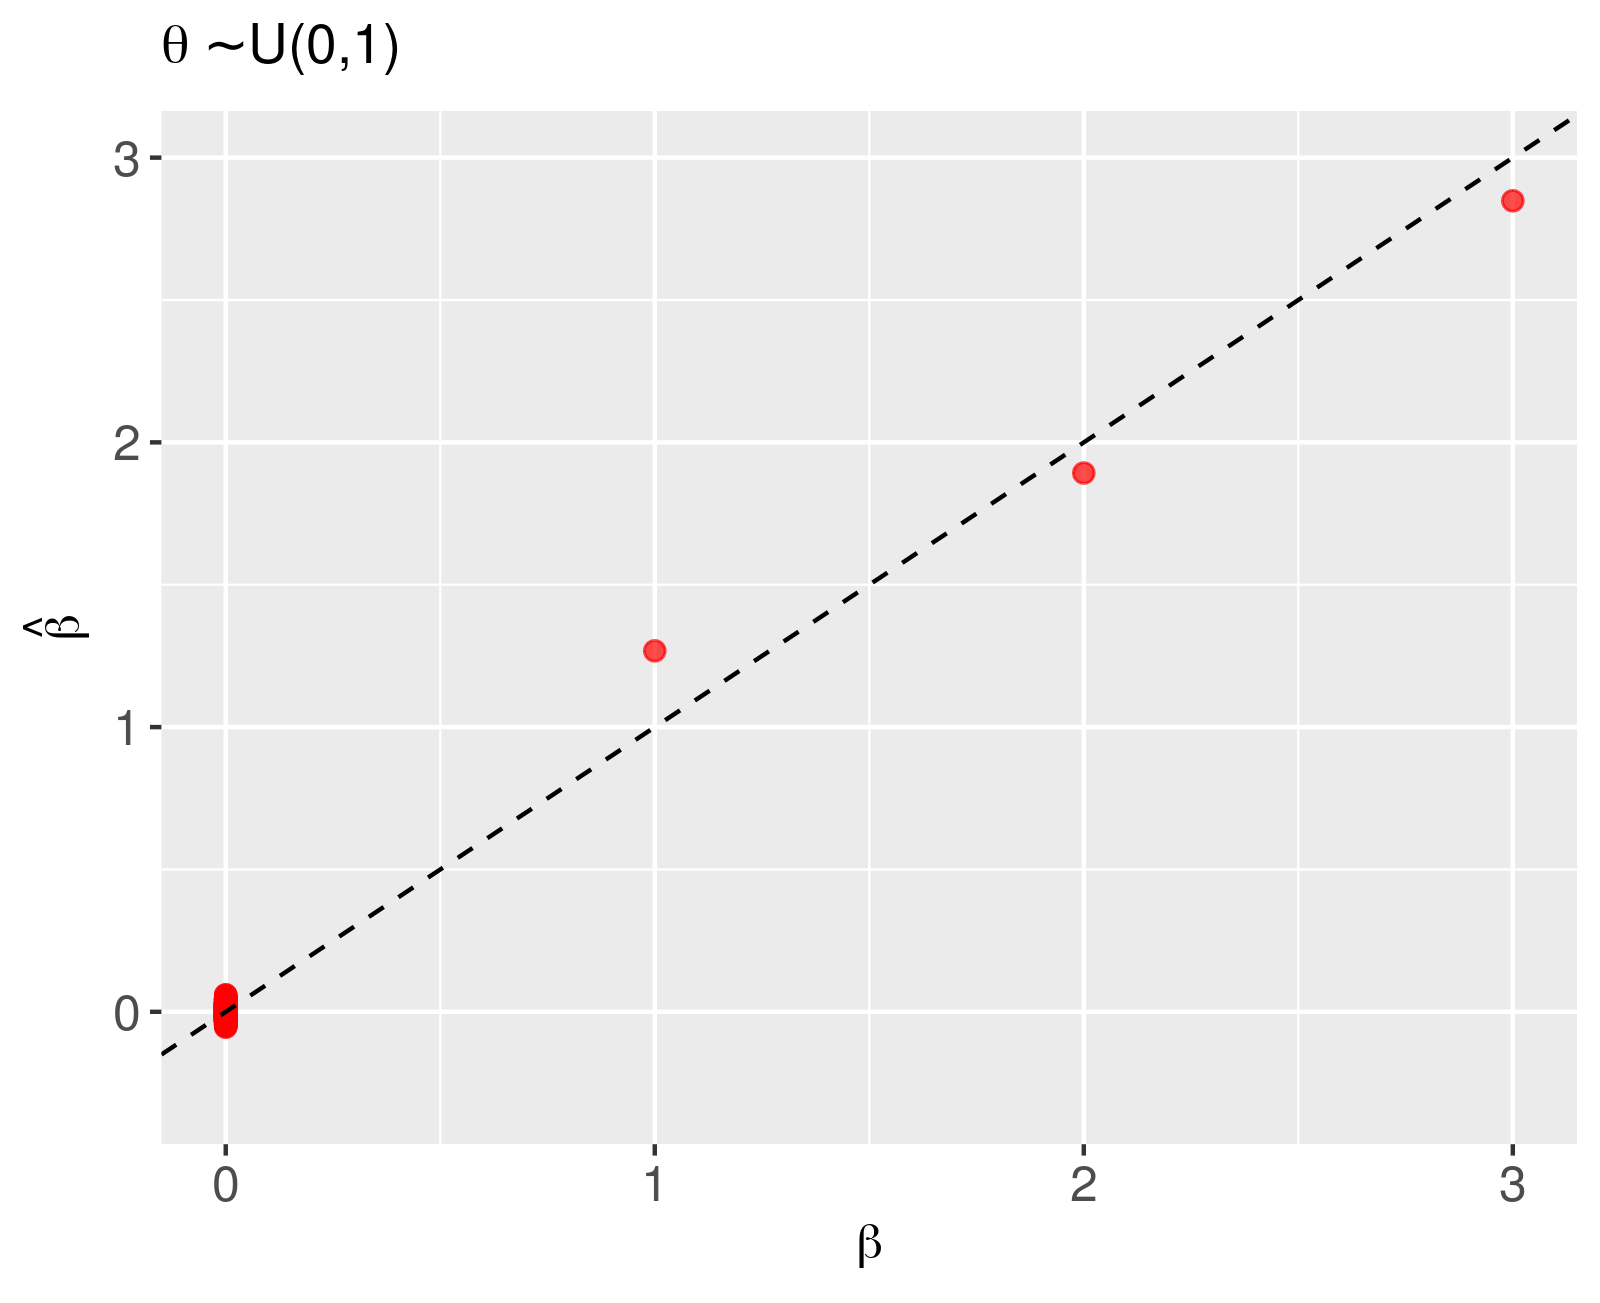
\includegraphics[width=0.7\linewidth]{images/fig1-a} 

}

\caption{Modal estimates of the regression coefficients}\label{fig:fig1-a}
\end{figure}
\begin{figure}

{\centering 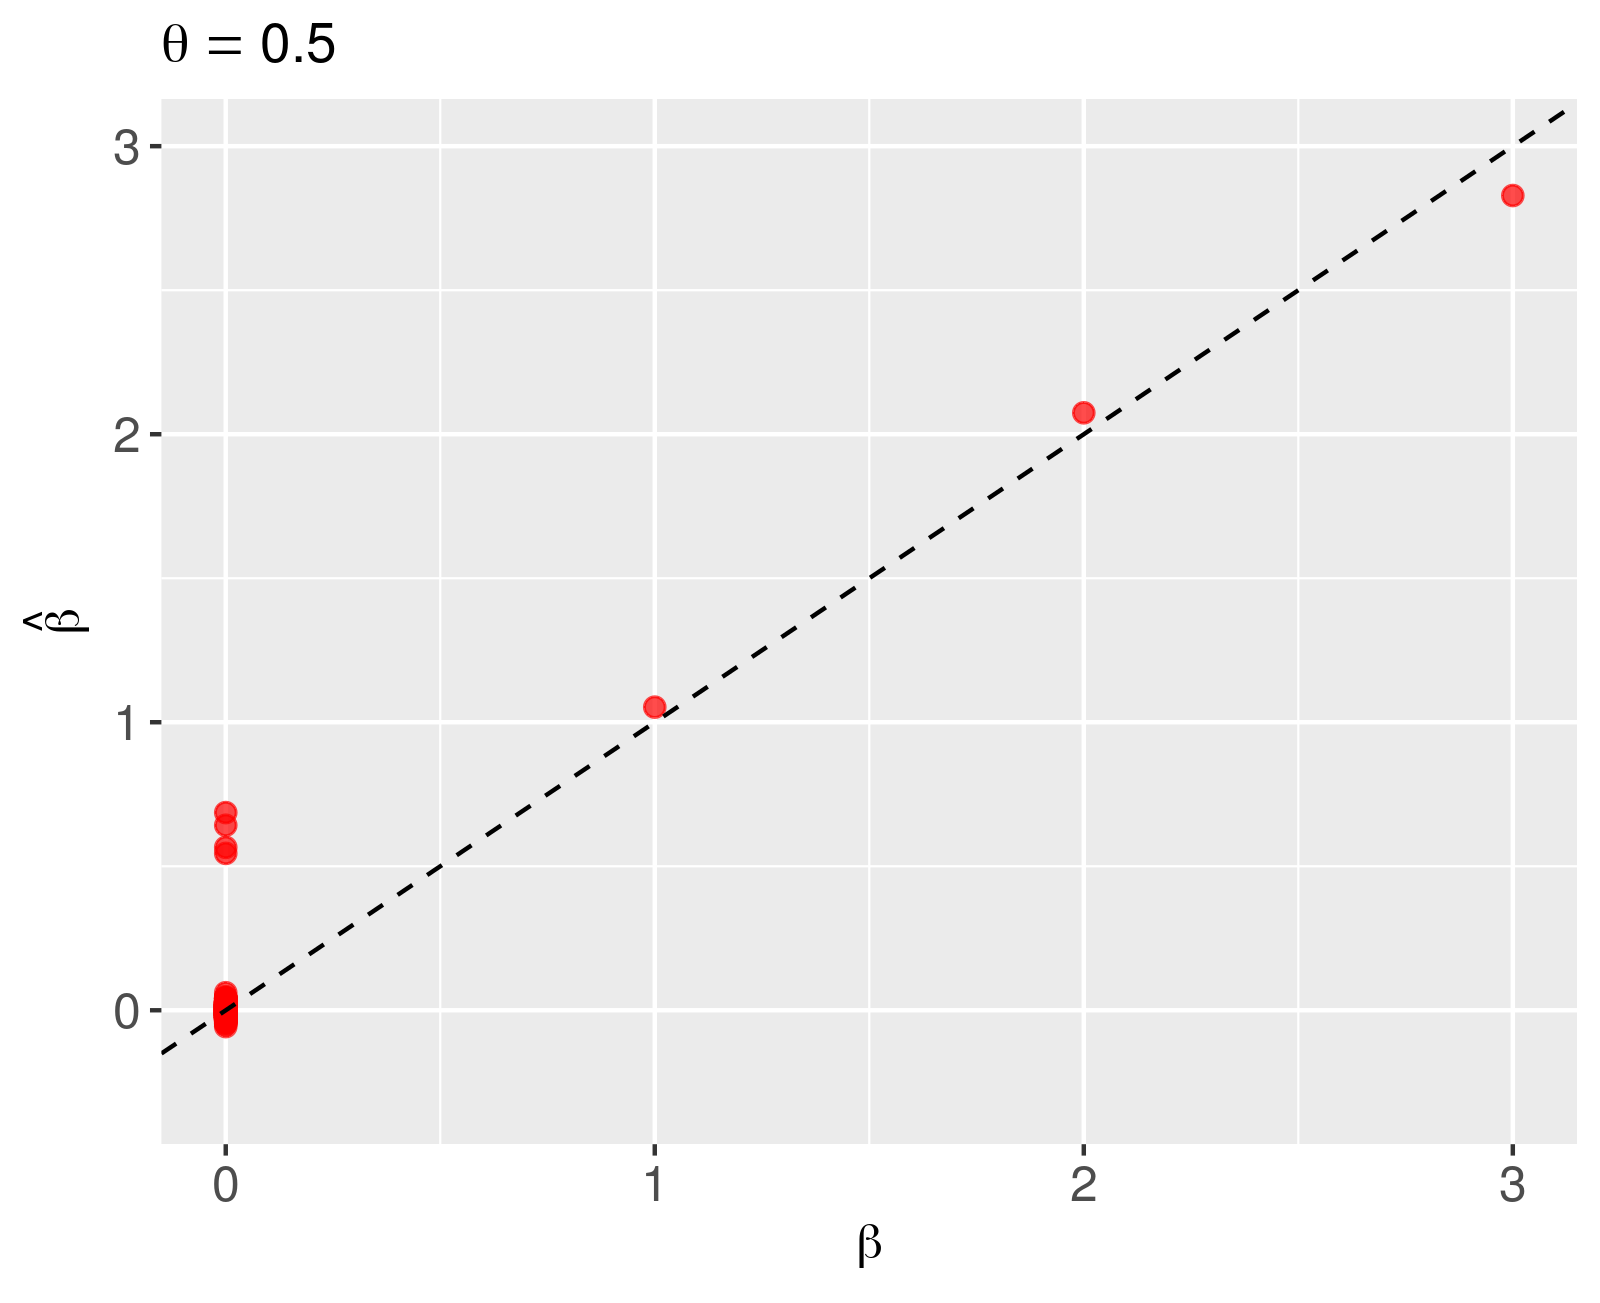
\includegraphics[width=0.7\linewidth]{images/fig1-b} 

}

\caption{Modal estimates of the regression coefficients}\label{fig:fig1-b}
\end{figure}

\hypertarget{the-effect-of-different-nu_0-and-boldsymbol-beta0-values-on-variable-selection}{%
\subsection{\texorpdfstring{The effect of different \(\nu_0\) and \({\boldsymbol \beta}^{(0)}\) values on variable selection}{The effect of different \textbackslash{}nu\_0 and \{\textbackslash{}boldsymbol \textbackslash{}beta\}\^{}\{(0)\} values on variable selection}}\label{the-effect-of-different-nu_0-and-boldsymbol-beta0-values-on-variable-selection}}

Rather than fixing \(\nu_0\) as 0.5, I vary it from 0 to 0.5 to see its effect on the variable selection. I imitate the author's method to consider the grid of \(\nu_0\) values \(V=\{0.01+k\times 0.01:k=0,\ldots,50\}\) again with \(\nu_1=1000\) fixed and \({\boldsymbol \beta}^{(0)}=\bf{1}_p\). Figure \ref{fig:fig2} shows the modal estimates of regression coefficients obtained for each \(\nu_0\in V\). We can discover that only when \(\nu_0 >0.15\), we can get a good estimation for the \({\boldsymbol \beta}\).I also consider the effect different initial values of \({\boldsymbol \beta}\) on the variable selection. Fix \(\nu_0=0.5\) and \(\nu_1=1000\), I set the grid of \({\boldsymbol \beta}^{(0)}=\bf{c}_p\) where \(\bf{c}\) is a p-dimension vector with each value \(c_i = \{-5+0.2\times k:k=0,\ldots,50\}, i=1,2,\ldots,p\). Figure \ref{fig:fig3} depicts modal estimates of regression coefficients with different initial values of \({\boldsymbol \beta}^{(0)}\). We discover only when \(|{\boldsymbol \beta}^{(0)}|<2\), we can get good estimation for the \({\boldsymbol \beta}\).

I also consider the effect different initial values of \({\boldsymbol \beta}\) on the variable selection. Fix \(\nu_0=0.5\) and \(\nu_1=1000\), I set the grid of \({\boldsymbol \beta}^{(0)}=\bf{c}_p\) where \(\bf{c}\) is a p-dimension vector with each value \(c_i = \{-5+0.2\times k:k=0,\ldots,50\}, i=1,2,\ldots,p\). Figure \ref{fig:fig3} depicts modal estimates of regression coefficients with different initial values of \({\boldsymbol \beta}^{(0)}\). We discover only when \(|{\boldsymbol \beta}^{(0)}|<2\), we can get good estimation for the \({\boldsymbol \beta}\).

\begin{figure}

{\centering 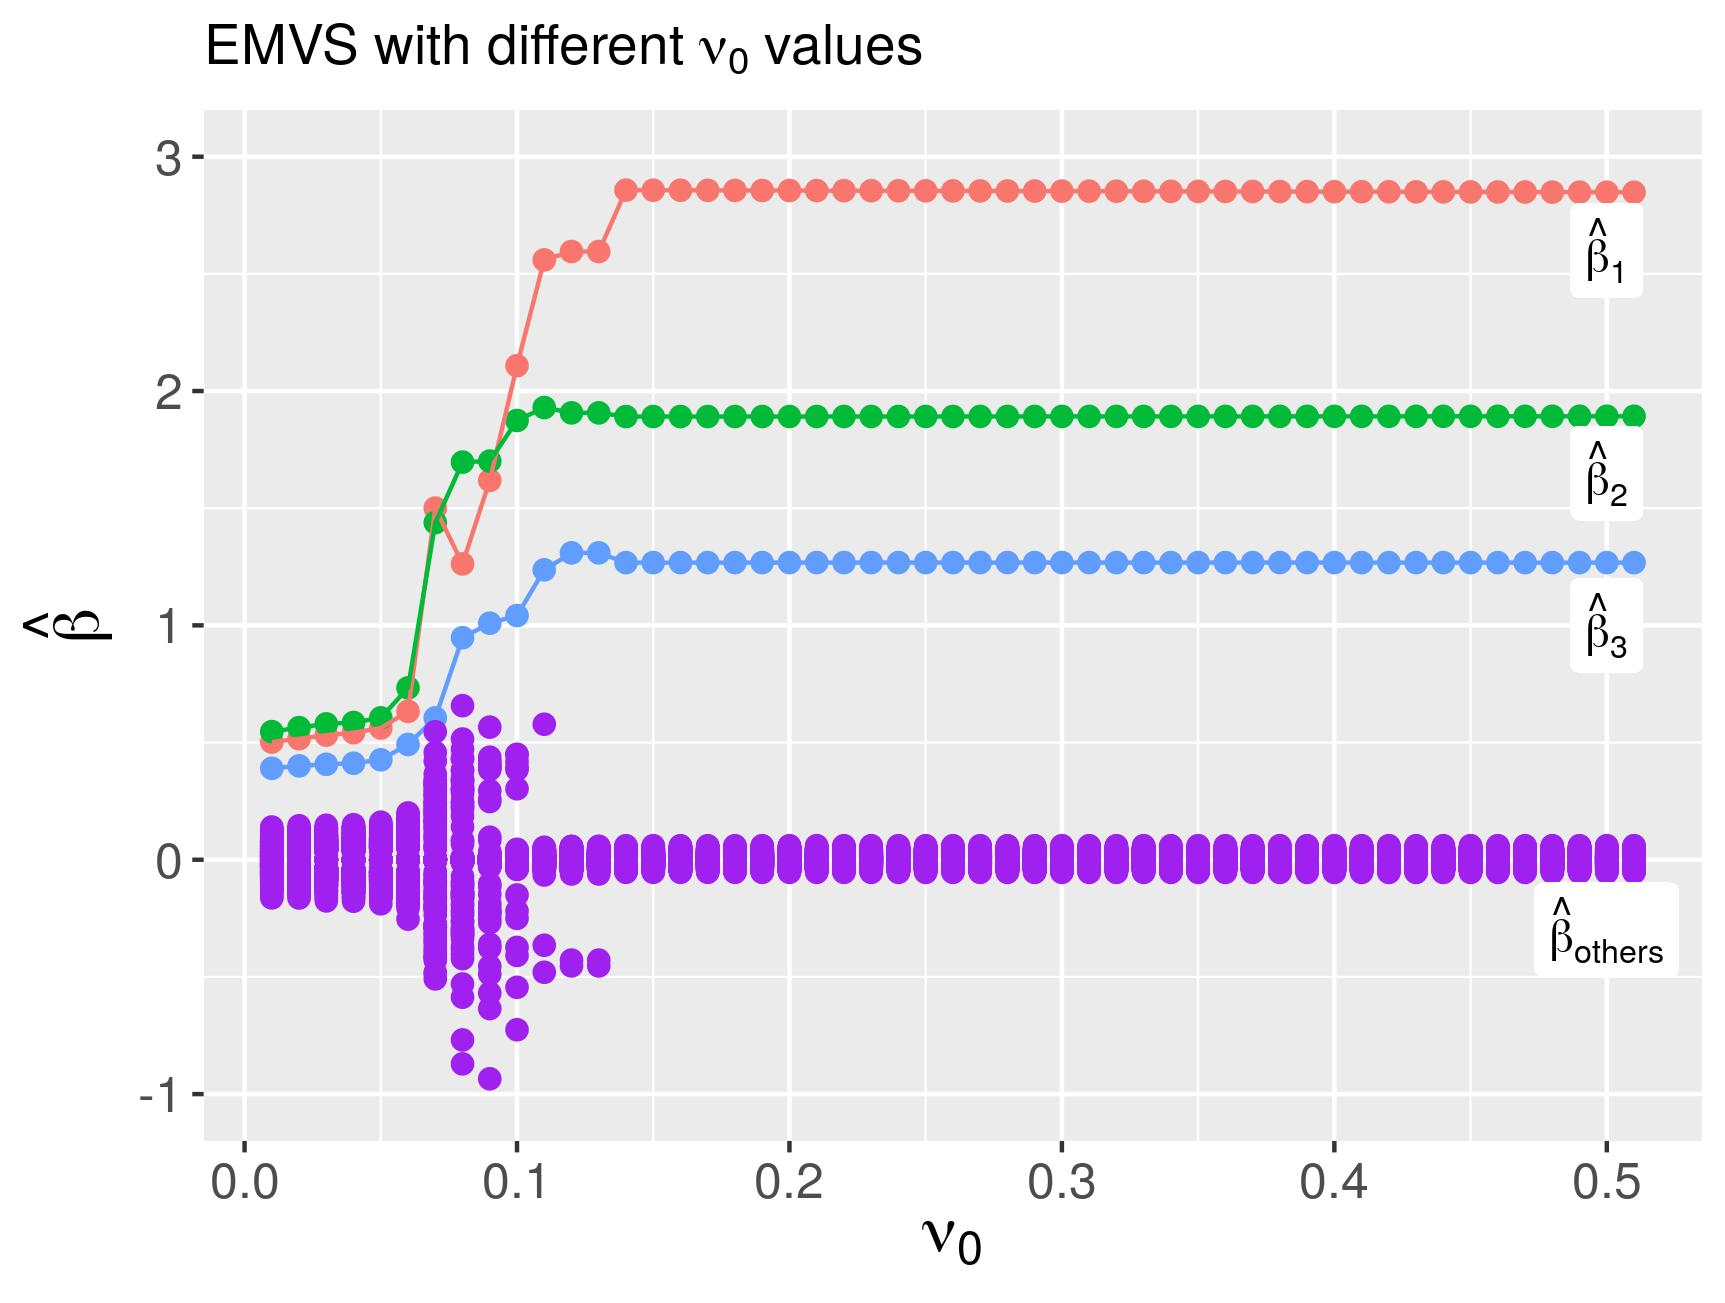
\includegraphics[width=0.7\linewidth]{images/fig2} 

}

\caption{Modal estimates of the regression coefficients}\label{fig:fig2}
\end{figure}
\begin{figure}

{\centering 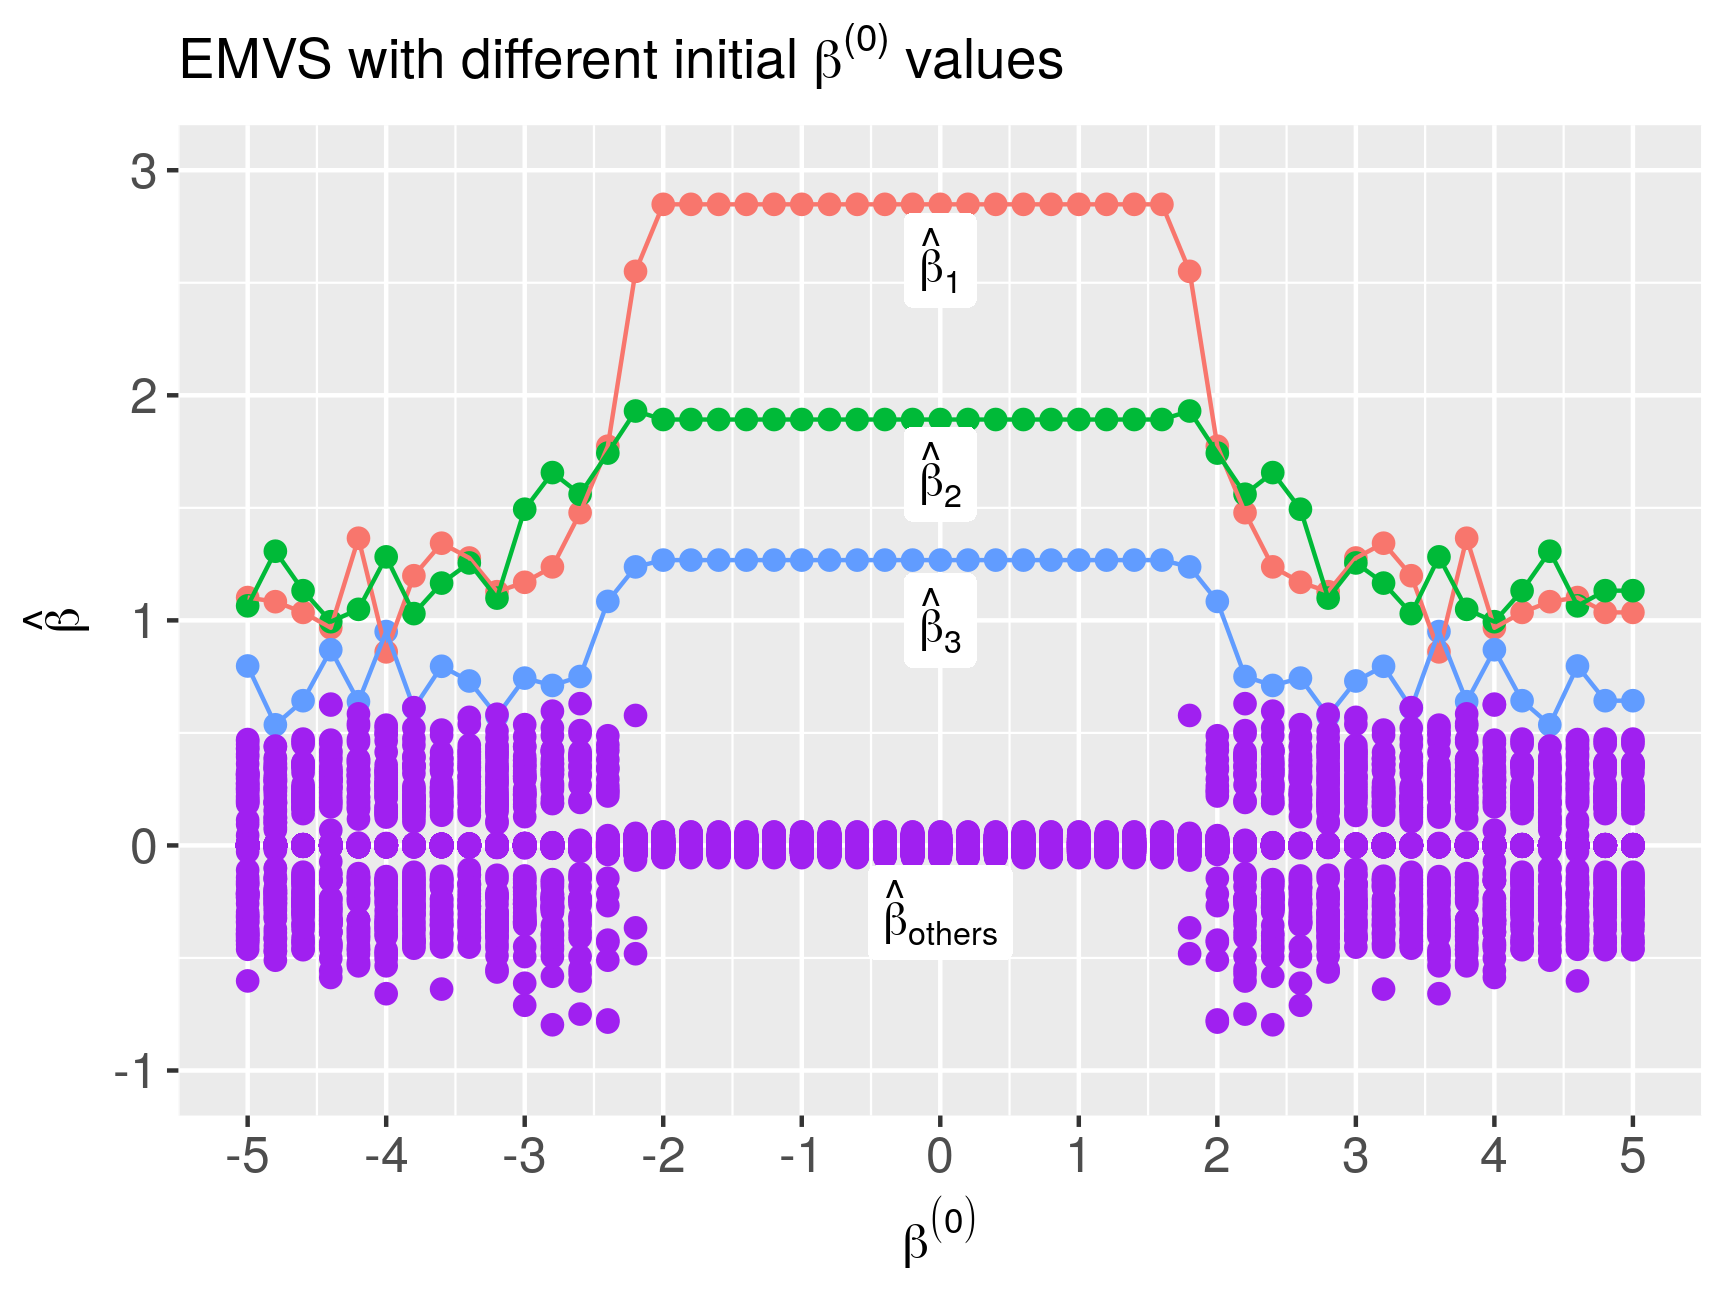
\includegraphics[width=0.7\linewidth]{images/fig3} 

}

\caption{Modal estimates of the regression coefficients}\label{fig:fig3}
\end{figure}

\bibliography{book.bib}


\end{document}
